% =====================================================================
% Sources of truth:
%   systemf.agda   the 72 registered rules and the 9 unregistered lemmas
%   closure.agda   the eight refl assertions certifying the absences
%   TRS.md         the rule-by-rule provenance table
%   supplement/    the generator, the POPLmark development, the TRS export
% Figures are extracted by agdatex from the marker regions in systemf.agda
% and examples.agda; blank lines inside an indented or opaque marker region
% break AgdaAlign, so do not insert any.
% =====================================================================
\documentclass[sigplan,anonymous,review]{acmart}
\usepackage{microtype}
% acmart already defines \Bbbk (via newtxmath); amssymb then refuses to
% redefine it.  Let it through rather than dropping amssymb.
\let\Bbbk\relax
\usepackage{amsmath,amssymb}
\usepackage{stmaryrd}
\usepackage{cleveref}  % was MISSING: every \Cref rendered as raw label text

\usepackage{Agda}

\usepackage{dsfont}
\usepackage{newunicodechar}
\newunicodechar{λ}{\ensuremath{\mathnormal\lambda}}
\newunicodechar{σ}{\ensuremath{\mathnormal\sigma}}
\newunicodechar{τ}{\ensuremath{\mathnormal\tau}}
\newunicodechar{π}{\ensuremath{\mathnormal\pi}}
\newunicodechar{ℕ}{\ensuremath{\mathbb{N}}}
\newunicodechar{∷}{\ensuremath{::}}
\newunicodechar{≡}{\ensuremath{\equiv}}
\newunicodechar{≅}{\ensuremath{\cong}}
\newunicodechar{∀}{\ensuremath{\forall}}
\newunicodechar{ᴸ}{\ensuremath{^L}}
\newunicodechar{ᴿ}{\ensuremath{^R}}
\newunicodechar{ʳ}{\ensuremath{^r}}
\newunicodechar{ᶻ}{\ensuremath{^Z}}
\newunicodechar{ₗ}{\ensuremath{_l}}
\newunicodechar{ⱽ}{\ensuremath{^V}}
\newunicodechar{⟧}{\ensuremath{\rrbracket}}
\newunicodechar{⟦}{\ensuremath{\llbracket}}
\newunicodechar{⊤}{\ensuremath{\top}}
\newunicodechar{⊥}{\ensuremath{\bot}}
\newunicodechar{₁}{\ensuremath{_1}}
\newunicodechar{₂}{\ensuremath{_2}}
\newunicodechar{₃}{\ensuremath{_3}}
\newunicodechar{₄}{\ensuremath{_4}}
\newunicodechar{₅}{\ensuremath{_5}}
\newunicodechar{₆}{\ensuremath{_6}}
\newunicodechar{₇}{\ensuremath{_7}}
\newunicodechar{₈}{\ensuremath{_8}}
\newunicodechar{₉}{\ensuremath{_9}}
\newunicodechar{∈}{\ensuremath{\in}}
\newunicodechar{₀}{\ensuremath{_0}}
\newunicodechar{′}{\ensuremath{'}}
\newunicodechar{ˢ}{\ensuremath{^S}}
\newunicodechar{ᴬ}{\ensuremath{^A}}
\newunicodechar{∘}{\ensuremath{\circ}}
\newunicodechar{𝟙}{\ensuremath{\mathds{1}}}  
\newunicodechar{𝟘}{\ensuremath{\mathds{O}}}
% \newunicodechar{𝟙}{\ensuremath{\mathbb{I}}}  
% \newunicodechar{𝟘}{\ensuremath{\mathbb{O}}}
\newunicodechar{ᴾ}{\ensuremath{^P}}
\newunicodechar{ᵀ}{\ensuremath{^T}}
\newunicodechar{⊎}{\ensuremath{\uplus}}
\newunicodechar{ι}{\ensuremath{\iota}}
\newunicodechar{⇐}{\ensuremath{\Leftarrow}}
\newunicodechar{⇒}{\ensuremath{\Rightarrow}}
\newunicodechar{➙}{\ensuremath{\to^P}}
\newunicodechar{Δ}{\ensuremath{\Delta}}
\newunicodechar{∅}{\ensuremath{\emptyset}}
\newunicodechar{⁺}{\ensuremath{^+}}
\newunicodechar{𝕏}{\ensuremath{\mathbb{X}}}
%\newunicodechar{·}{\ensuremath{\cdot}} %seems to be defined already!
\newunicodechar{∙}{\ensuremath{\cdot}}
\newunicodechar{⁇}{\ensuremath{?}}
\newunicodechar{‼}{\ensuremath{!}}
\newunicodechar{⊕}{\ensuremath{\oplus}}
\newunicodechar{ℤ}{\ensuremath{\mathbb{Z}}}
\newunicodechar{μ}{\ensuremath{\mu}}
\newunicodechar{∃}{\ensuremath{\exists}}
\newunicodechar{；}{\ensuremath{\fatsemi}}
\newunicodechar{Σ}{\ensuremath{\Sigma}}
\newunicodechar{ᴿ}{\ensuremath{^R}}
\newunicodechar{ᵢ}{\ensuremath{_i}}
\newunicodechar{≢}{\ensuremath{\nequiv}}
\newunicodechar{≟}{\ensuremath{\stackrel{{\tiny?}}{=}}}
\newunicodechar{≤}{\ensuremath{\le}}
\newunicodechar{ᵇ}{\ensuremath{^b}}
\newunicodechar{𝓣}{\ensuremath{\mathcal{T}}}
\newunicodechar{𝓔}{\ensuremath{\mathcal{E}}}
\newunicodechar{Γ}{\ensuremath{\Gamma}}
\newunicodechar{γ}{\ensuremath{\gamma}}
\newunicodechar{⊔}{\ensuremath{\sqcup}}
\newunicodechar{α}{\ensuremath{\alpha}}
\newunicodechar{η}{\ensuremath{\eta}}
\newunicodechar{ω}{\ensuremath{\omega}}
\newunicodechar{◁}{\ensuremath{\lhd}}
%PT: seems to be already defined
%\newcommand{\lambdabar}{{\mkern0.75mu\mathchar '26\mkern -9.75mu\lambda}}
\newunicodechar{ƛ}{\ensuremath{\lambdabar}}
\newunicodechar{Λ}{\ensuremath{\mathnormal\Lambda}}
\newunicodechar{ρ}{\ensuremath{\rho}}
\newunicodechar{𝓖}{\ensuremath{\mathcal{G}}}
\newunicodechar{ℓ}{\ensuremath{\ell}}
\newunicodechar{♯}{\ensuremath{\sharp}}
\newunicodechar{⇓}{\ensuremath{\Downarrow}}
\newunicodechar{𝓥}{\ensuremath{\mathcal{V}}}
\newunicodechar{∧}{\ensuremath{\wedge}}
\newunicodechar{ₛ}{\ensuremath{_s}}
\newunicodechar{χ}{\ensuremath{\chi}}
\newunicodechar{⊨}{\ensuremath{\models}}
\newunicodechar{⦂}{\ensuremath{\mathbf{:}}}
\newunicodechar{ς}{\ensuremath{\varsigma}}
\newunicodechar{𝓓}{\ensuremath{\mathcal{D}}}
\newunicodechar{∎}{\ensuremath{\square}}
\newunicodechar{■}{\ensuremath{\blacksquare}}
\newunicodechar{↠}{\ensuremath{\twoheadrightarrow}}
\newunicodechar{↪}{\ensuremath{\hookrightarrow}}
\newunicodechar{ⁱ}{\ensuremath{^i}}
\newunicodechar{Π}{\ensuremath{\Pi}}
\newunicodechar{∋}{\ensuremath{\ni}}
\newunicodechar{∍}{\ensuremath{\ni}}
\newunicodechar{‵}{\ensuremath{`}}
\newunicodechar{⨆}{\ensuremath{\bigsqcup}}
\newunicodechar{δ}{\ensuremath{\delta}}
\newunicodechar{κ}{\ensuremath{\kappa}}
\newunicodechar{⦃}{\ensuremath{\{\!|}}  % \lBrace from stix
\newunicodechar{⦄}{\ensuremath{|\!\}}}  % \rBrace from stix
\newunicodechar{⌊}{\ensuremath{\lfloor}}
\newunicodechar{⌋}{\ensuremath{\rfloor}}
\newunicodechar{𝟎}{\ensuremath{\mathbf{0}}}
\newunicodechar{𝟏}{\ensuremath{\mathbf{1}}}
\newunicodechar{𝟐}{\ensuremath{\mathbf{2}}}
\newunicodechar{β}{\ensuremath{\beta}}
\newunicodechar{≥}{\ensuremath{\geq}}
\newunicodechar{ₒ}{\ensuremath{_o}}
\newunicodechar{∊}{\ensuremath{\in}}
\newunicodechar{;}{\ensuremath{;}}
\newunicodechar{⋯}{\ensuremath{\mkern2mu \cdotp \mkern-2mu \cdotp \mkern-2mu \cdotp \mkern1mu }}
\newunicodechar{⊢}{\ensuremath{\vdash}}
\newunicodechar{∶}{\ensuremath{:}}
\newunicodechar{★}{\ensuremath{\star}}
\newunicodechar{ᴷ}{\ensuremath{^K}}
\newunicodechar{ϕ}{\ensuremath{\varphi}}
\newunicodechar{ᴮ}{\ensuremath{^B}}
\newunicodechar{＋}{}
\newunicodechar{ᵣ}{\ensuremath{_r}}
\newunicodechar{ₓ}{\ensuremath{_x}}
\newunicodechar{ₜ}{\ensuremath{_t}}
\newunicodechar{𝓡}{\ensuremath{\mathcal{R}}}
\newunicodechar{𝓢}{\ensuremath{\mathcal{S}}}
\newunicodechar{𝓚}{\ensuremath{\mathcal{K}}}
\newunicodechar{ᴹ}{\ensuremath{^M}}
\newunicodechar{ᵗ}{\ensuremath{^t}}
\newunicodechar{ξ}{\ensuremath{\xi}}
\newunicodechar{≐}{\ensuremath{\doteq}}
\newunicodechar{⸴}{\ensuremath{,}}
\newunicodechar{ᴱ}{\ensuremath{^E}}
\newunicodechar{⨟}{\ensuremath{\fatsemi}}
\newunicodechar{𝒜}{\ensuremath{\mathcal{A}}}
\newunicodechar{𝒮}{\ensuremath{\mathcal{S}}}
\newunicodechar{∪}{\ensuremath{\cup}}
\newunicodechar{∨}{\ensuremath{\lor}}
\newunicodechar{•}{\ensuremath{\bullet}}\newunicodechar{═}{\ensuremath{=}}
\newunicodechar{ᵛ}{\ensuremath{^v}}
\newunicodechar{⇑}{\ensuremath{\Uparrow}}

\input{agdamacros}

\definecolor{agdablue}{HTML}{0000CD}
\DisableLigatures[-]{encoding=T1}
\newcommand{\bsym}[1]{\textcolor{agdablue}{#1}}
\newcommand{\tdot}{\mkern2mu \textcolor{agdablue}{\cdotp} \mkern-2mu \textcolor{agdablue}{\cdotp} \mkern-2mu \textcolor{agdablue}{\cdotp} \mkern1mu}

%% ═══ REVISION MARKERS.  Currently unused: wrap a passage in \RW{} to flag
%% it, or drop a \Stale / \AddHere / \Nota note.  pagecheck.sh strips them. ═
\usepackage{tikz}
\definecolor{staleC}{HTML}{B3261E}
\definecolor{addC}{HTML}{15507D}
\definecolor{notaC}{HTML}{8A6116}
\newcommand{\Stale}[1]{{\color{staleC}\sffamily\bfseries\small$\blacktriangleright$\,STALE: #1}}
\newcommand{\AddHere}[1]{{\color{addC}\sffamily\bfseries\small$\blacktriangleright$\,ADD: #1}}
\newcommand{\Nota}[1]{{\color{notaC}\sffamily\bfseries\small$\blacktriangleright$\,NOTATION: #1}}
\definecolor{rewC}{HTML}{1B7A3E}
\newcommand{\RW}[1]{{\color{rewC}#1}}
\newcommand{\RWnote}[1]{{\color{rewC}\sffamily\bfseries\small$\blacktriangleright$\,REWRITTEN: #1}}
\newcommand{\MarkBlock}[2]{%
  \par\smallskip\noindent\textcolor{#1}{\rule{\linewidth}{0.9pt}}

  \par\nopagebreak\noindent{\color{#1}\sffamily\footnotesize #2}

  \par\nopagebreak\noindent\textcolor{#1}{\rule{\linewidth}{0.9pt}}\par\smallskip}

\setcopyright{none}
\acmConference[CPP '27]{Certified Programs and Proofs}{2027}{}
\acmDOI{XXXXXXX.XXXXXXX}
\settopmatter{printacmref=false}

\begin{document}

\title{Definitional Equalities for the Substitution Calculus using Rewrite Rules}

\author{Marius Weidner}
\email{weidner@cs.uni-freiburg.de}
\orcid{0009-0008-1152-165X}
\affiliation{%
      \institution{University of Freiburg}
      \city{Freiburg}
      \country{Germany}}

\keywords{Explicit Substitutions, Term Rewrite Systems, Agda}

\ccsdesc[300]{Theory of computation~Equational logic and rewriting}

\input{systemf}
\input{examples}

\begin{abstract}

      Choosing a representation of variable binding is a central problem in
      mechanizing programming language metatheory. De~Bruijn indices are
      canonical, but developments built on them accumulate lemmas about how
      substitutions compose and how they pass under binders, and every one of
      those lemmas has to be applied by hand or by a tactic.

      The $σ$-calculus makes parallel substitutions first-class and normalizes
      them by rewriting. Modeling substitutions as functions turns its rules into
      theorems, which is what libraries such as \textsc{Autosubst} exploit, but
      the resulting equalities stay propositional.

      We register the $σ$-calculus as rewrite rules in Agda, so that
      substitutions are normalized during conversion rather than by a tactic.
      Two requirements pull against each other. The rules are provable only if
      the primitives compute, and eligible for rewriting only if they are stuck.
      Opaque definitions satisfy both. We identify which variant of the calculus
      can be oriented at all, since native inductive variables and surjective
      pairing cannot coexist in one rewrite system, and derive the rule set that
      follows. A generator emits it from a syntax description. Agda certifies
      local confluence and AProVE termination. Solving the POPLmark Challenge
      and POPLmark Reloaded on top exercises the result. The laws we cannot
      register are never needed, and a single law resists our orientation.
\end{abstract}

\maketitle

\section{Introduction}\label{sec:introduction}

Effectively handling variable binding remains a central challenge when
mechanizing programming language metatheory. Compared to pen-and-paper proofs,
binders in proof assistants are a notorious source of uninteresting
technicalities and boilerplate, and many representations have been proposed to
contain them, among them locally nameless binders, nominal
syntax~\cite{10.1007/11532231_4, Nominal2-AFP}, higher-order abstract syntax,
and de~Bruijn indices. De~Bruijn syntax is canonical and easy
to define, but a development built on it still pays for a long list of lemmas
about substitution composition and about the interaction of substitution with
binders.

On paper, substitution usually replaces a single variable. In a proof assistant
one instead works with parallel substitutions, which map variables to terms and
replace all of them at once. The $σ$-calculus~\cite{10.1145/96709.96712} makes
such a map a first-class object with primitive operations for identity,
weakening, extension, composition and lifting, together with a rewrite system
that normalizes expressions built from them. The de~Bruijn algebra, which models
substitutions as functions, provides a semantic model in which those rules
become provable~\cite{schafer2015autosubst}, and hence usable for equational
reasoning. \textsc{Autosubst}~\cite{schafer2015autosubst} and its successor
\textsc{Autosubst 2}~\cite{10.1145/3293880.3294101} generate the operations,
the proofs of the laws, and a tactic that normalizes substitutions inside a
goal. \textsc{Autosubst 2} additionally supports intrinsically scoped syntax,
packages substitutions over several sorts into vectors, and promotes renamings,
the substitutions that map variables to variables, to first-class citizens of
the equational theory.

The equalities so obtained are propositional. Normalization is a step the user
takes, and every goal that mentions a substitution has to be brought into normal
form before it can be closed. Recent support for user-defined rewrite rules in
Agda~\cite{cockx:LIPIcs.TYPES.2019.2, 10.1145/3434341} and
Rocq~\cite{leray_et_al:LIPIcs.ITP.2024.26} offers to remove that step by
promoting propositional equalities to definitional ones. Consistency is retained
as long as the registered rules are supported by proofs and the resulting system
is confluent and terminating~\cite{10.1145/3434341}. A syntactic condition comes
with it. Agda applies a rule by higher-order pattern
unification~\cite{10.1007/978-3-642-21691-6_5} against its left-hand side, and
therefore demands that this side be stuck on a defined symbol.

\emph{Functions or constructors.} There are two ways to model a parallel
substitution, and the syntactic condition tells them apart. Modeled as
functions, the primitives compute, so the laws are provable, but composition
unfolds to a lambda abstraction and no left-hand side is ever stuck. Modeled as
syntax, with extension a term former, every left-hand side is stuck by
construction. This is the route Wadler takes, and it avoids renamings
altogether~\cite{Wadler_2024}. What it costs is that a constructor has nothing
to compute, so the rule $x\,[\,\bsym{\mathsf{wk}}\,] = \bsym{\mathsf{suc}}\,x$ is
no longer derivable, a variable acquires two inequivalent representations, and
every law that pushes weakening through a term stays propositional. Agda's
opaque definitions~\cite{gratzer2022controlling} give both properties at once.
An opaque symbol is stuck outside its block and computes inside it, so one
definition can carry the proof of a law and also head that law's left-hand side.

\emph{Which calculus can be oriented.} Not every version of the $σ$-calculus is
a candidate. The original~\cite{10.1145/96709.96712} is confluent on ground
terms but not on open ones, and open terms, those with metavariables, are the
setting of any mechanized development. The two variants that repair this differ
on the $η$-laws, that is on surjective pairing, and the choice is forced for us.
The complete variant $σ_{SP}$~\cite{Stark:2020:Mechanising,
10.1145/2676724.2693163} can afford $η$ only because it has no numerals, since
the variable $n$ \emph{is} the expression $0\,[\,\bsym{\mathsf{wk}}\,]^n$. A scoped
syntax in a proof assistant has native inductive variables instead, and having
them forces $x\,[\,\bsym{\mathsf{wk}}\,] = \bsym{\mathsf{suc}}\,x$, which
identifies the two spellings of a variable and thereby destroys the left-hand
side of $η$, which mentions its substitution twice and is not left-linear.
Native inductive variables and surjective pairing cannot coexist in one rewrite
system. We keep the variables and drop $η$, and so build on
$σ_\Uparrow$~\cite{10.1145/226643.226675, HMP98}, whose detail \cref{sec:pre-sig}
gives. Adding the two $η$-laws to our rule set is refuted for confluence by
three independent tools (\cref{sec:ext}), exactly as this argument predicts.

\subsection*{Contributions}

\begin{itemize}
      \item \textbf{A rewrite system.} The $σ$-calculus with first-class
            renamings, made definitional in a multi-sorted, intrinsically scoped
            setting. Every rule is proved before it is registered, so logical
            consistency is preserved. We derive the rule set rather than list
            it, as a small base closed under three completion operators, each
            carrying a side condition that says when an image is not needed, so
            that the absences are predicted as well as the rules.
      \item \textbf{Machine-checked metatheory of the rule set.} Agda certifies
            local confluence, and AProVE proves termination and confluence of
            the first-order export. Both hold at two signature sizes, which is
            evidence that what is proved is a property of the schema rather than
            of one language.
      \item \textbf{A generator.} A single-file tool that emits the entire
            infrastructure from a higher-order abstract syntax description.
      \item \textbf{An evaluation at scale.} The POPLmark Challenge, Parts 1A,
            1B, 2A, 2B and~3, and POPLmark Reloaded, solved on generated cores.
            The laws we cannot register are never needed. One law resists our
            orientation, and we can say exactly why.
\end{itemize}

\subsection*{Structure}

\Cref{sec:pre} reviews Agda's rewrite rules and opaque blocks, our scoped
syntax, and the $σ$-calculus. \Cref{sec:mis} develops the rule set for System~F
and explains what makes it registrable. \Cref{sec:fwk} reports the generator,
the POPLmark evaluation, the external proofs, and future work. \Cref{sec:rwk}
discusses related work and \cref{sec:con} concludes.

\section{Preliminaries}\label{sec:pre}

We review the two Agda features the construction rests on, the scoped syntax we
use, and the $σ$-calculus itself. All Agda code shown in this paper is in the
supplement.

\subsection{Agda and Relevant Language Features}\label{sec:pre-agd}

Agda is a dependently typed functional language and proof assistant based on
Martin-Löf type theory~\cite{MARTINLOF197573}, where proofs are verified by type
checking. Proofs are significantly easier when terms are \emph{definitionally
equal}, that is, when they reduce to the same term. When they are not, users
must resort to manual equational reasoning with propositional equality, which is
cumbersome as Agda lacks automated proof-discharge tactics. Maximizing
definitional equalities thus directly reduces manual effort. Beyond standard
features such as indexed inductive types and dependent pattern
matching~\cite{10.1145/3236770}, this work rests on two more advanced ones.

\subsection*{Rewrite Rules}
User-defined rewrite rules~\cite{10.1145/3434341, cockx:LIPIcs.TYPES.2019.2}
extend Agda's normalization-by-evaluation approach for definitional equalities
by treating propositional equalities as reduction rules. A proof of
$\AgdaFunction{f}\, p_1 \ldots p_n \AgdaFunction{≡} v$ is eligible if
\AgdaFunction{f} is a postulate, defined function or constructor, if every
variable bound in the statement occurs in a pattern position among $p_1, \ldots,
p_n$, and if the left-hand side is stuck. For example, the right identity of
addition qualifies:
\ERewrite{} Once it is registered via \ERewriteIt{}, Agda treats \AgdaBound{n}
\AgdaFunction{+} \AgdaNumber{0} as definitionally equal to \AgdaBound{n}:
\ERewriteEx{}

Beyond the syntactic restriction, the rule set as a whole has to be well behaved.
We rely throughout on the following, which is the criterion under which Agda's
rewrite rules are known to be sound~\cite{10.1145/3434341}.

\begin{quote}\itshape
      If every registered rule is inhabited by a proof of the corresponding
      propositional equality, and the resulting rewrite system is confluent and
      terminating, then adding it preserves consistency and subject reduction.
\end{quote}

\noindent We discharge the three obligations separately. Every rule is proved
before it is registered (\cref{sec:mis-sig}); Agda's
\texttt{--local-confluence-check} joins every critical pair; and termination is
established externally (\cref{sec:ext}), which with local confluence gives
confluence by Newman's lemma. Termination is the obligation that has to leave
Agda, because Agda never checks it: a non-terminating rule set simply makes the
type checker loop.

\subsection*{Opaque Blocks}
Opaque definitions~\cite{gratzer2022controlling} let the user treat code as
non-unfolding symbols. A definition inside an \AgdaKeyword{opaque} block is
visible but does not reduce outside it, and the \AgdaKeyword{unfolding} keyword
exposes its computational behavior where that is wanted. The feature exists to
improve type checking times, since ordinarily one wants everything to unfold.
Here it serves the opposite purpose. Declaring the substitution primitives opaque
makes them stuck symbols and thereby qualifies them for rewriting, while the
proofs of the rules unfold them and use their computational behavior.

\subsection{Multi-Sorted and Scoped Syntax}\label{sec:pre-syn}
\begin{figure*}[t]
      \begin{minipage}[t]{0.44\linewidth}
            \raggedright{}
            \EScoped{}
      \end{minipage}
      \hfill
      \begin{minipage}[t]{0.52\linewidth}
            \raggedright{}
            \EMultiSorted{}
            \EMultiSortedTm{}
      \end{minipage}
      \caption{Classically Scoped vs. Multi-Sorted Scoped Syntax}\label{fig:pre-svm}
\end{figure*}

Many programming languages feature several syntactic categories. System~F~\cite{girard1972,
      10.1007/3-540-06859-7_148} has three: expressions, types, and
kinds\footnote{Kinding for System~F is trivial and could be omitted.}. We use
intrinsically scoped syntax to prevent the construction of ill-scoped terms.
\Cref{fig:pre-svm} (left) shows the standard implementation, where types are
indexed by the number of type variables, expressions by the numbers of type and
expression variables, and variables are de~Bruijn indices of type
\AgdaDatatype{Fin} \AgdaBound{n}.

Scoped syntax rules out scoping errors without committing to full intrinsic
typing, which is hard to work with for larger systems. It has one drawback. The
standard representation forces one substitution operation per pair of sorts, such
as type-in-type, type-in-expression and expression-in-expression. This is the
representation \textsc{Autosubst 2} chooses, and it explains why that system
needs vector substitutions, which bundle the substitutions over the different
sorts and come with normalization rules of their own.

To avoid this combinatorial explosion we unify the syntax along two orthogonal
dimensions, shown in \cref{fig:pre-svm} (right). Variables and terms form a
single datatype \AgdaBound{S} \AgdaDatatype{⊢[} \AgdaBound{m} \AgdaDatatype{]}
\AgdaBound{s}, indexed by a \AgdaDatatype{Mode} \AgdaBound{m}, a target
\AgdaDatatype{Sort} \AgdaBound{s} and a \AgdaDatatype{Scope} \AgdaBound{S}, a
list of sorts. Variables of type \AgdaBound{S} \AgdaDatatype{∋} \AgdaBound{s} are
represented across all sorts at once, the length of \AgdaBound{S} being the
number of variables in scope and the position of \AgdaBound{s} in \AgdaBound{S}
the de~Bruijn index. Renamings and substitutions defined over this syntax then
operate uniformly across sorts, and vector substitutions become unnecessary.

The mode index is more than a device for sharing definitions. A variable and a
term behave differently under a map. Renaming a variable yields a variable, which
the applied rules can match again, whereas substituting one yields a term, which
they cannot. Several rules therefore exist in two versions pointing in opposite
directions, and \cref{sec:mis-sig} shows where this is forced.

\subsection{A Short History of the Sigma Calculus}\label{sec:pre-sig}

Explicit-substitution calculi turn substitutions into syntax, so that
$t\,[\,σ\,]$ is a term and $σ$ itself can be composed, extended and pushed under
binders by rewriting. Three of them matter here.

$σ$~\cite{10.1145/96709.96712} is the original. Lifting is \emph{defined},
$\Uparrow σ := \bsym{\mathsf{zero}} \bsym{\cdot} (σ \bsym{⨟}
\bsym{\mathsf{wk}})$, and the two $η$-laws are part of the theory. Both versions
of \textsc{Autosubst} build on it.

$σ_\Uparrow$~\cite{10.1145/226643.226675, HMP98} keeps $\Uparrow$ primitive and
drops $η$, and thereby recovers confluence on open terms. Its 23 rules,
tabulated by Hardin et al.~\cite{HMP98}, fall into the applied rules, where
a variable meets a map, the traversal rules, one per constructor, the map
algebra, and a family of $\fatsemi$-companions that exists only because
associativity is oriented. This is the calculus we build on.

$σ_{SP}$~\cite{Stark:2020:Mechanising} adds the $η$-laws back and is thereby
complete, deciding every equality between substitution
expressions~\cite{10.1145/2676724.2693163}.

Primitive lifting and the absence of $η$ stand or fall together. Eliminate
lifting and $\mathsf{lift\text{-}id}$, $\Uparrow\bsym{\mathsf{id}} =
\bsym{\mathsf{id}}$, stops holding by computation, because $\Uparrow$ then
unfolds to $\bsym{\mathsf{zero}} \bsym{\cdot} (\bsym{\mathsf{id}} \bsym{⨟}
\bsym{\mathsf{wk}})$ and only $η\mathsf{\text{-}id}$ reconciles the two. As
\cref{sec:introduction} argued, $η$ is unavailable to us. Its left-hand side
$(\bsym{\mathsf{zero}}[σ]) \bsym{\cdot} (\bsym{\mathsf{wk}} \bsym{⨟} σ)$
mentions $σ$ twice, so any rule that rewrites one occurrence destroys the
pattern for the other, and $x\,[\,\bsym{\mathsf{wk}}\,] =
\bsym{\mathsf{suc}}\,x$ is such a rule. Completeness and orientability are
incompatible here, and a paper about rewriting gives up completeness. The price
is four laws, the two $η$-laws once for renamings and once for substitutions,
which we prove but do not register. \Cref{sec:eval} reports
what that costs in practice.

One further ingredient appears in none of these calculi. Defining instantiation
for a substitution requires pushing under binders, which requires weakening the
terms in the substitution, which is instantiation again, a loop no termination
checker accepts. The standard repair is to define renamings
first~\cite{10.1007/11617990_1}. \textsc{Autosubst 2} takes the further step of
making renamings first-class and extending the equational theory with rules that
relate the two worlds~\cite{10.1145/3293880.3294101}. The extended system is no
longer complete, and its confluence was left as a
conjecture~\cite{Stark:2020:Mechanising}. We do not settle that conjecture, since
the rule set we register is not theirs, but we answer the corresponding question
for a concrete two-world system in \cref{sec:ext}.

% The design-decision ladder: how the rule set was FOUND.
% Deliberately says nothing about which rules result -- the rule groups are
% Section 3.2's job, and putting them here forced arrows that crossed the
% branch labels and made the figure unreadable.
% Requires \usepackage{tikz} in the preamble.  Spans both columns (figure*).

\begin{figure*}
\centering
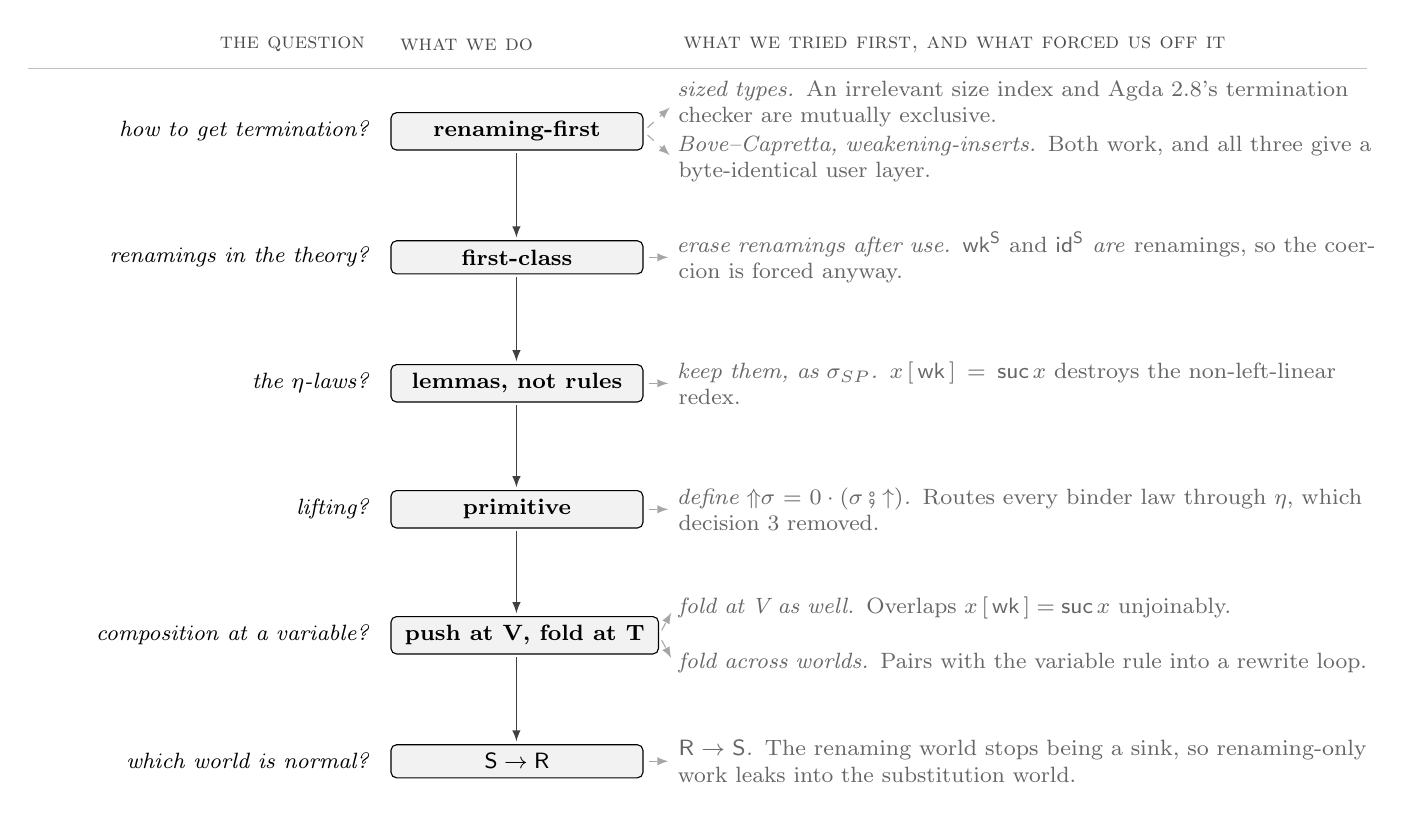
\begin{tikzpicture}[
    x=1mm, y=1mm,
    ask/.style   = {anchor=east, font=\footnotesize\itshape, inner sep=2pt},
    take/.style  = {draw, rounded corners=2pt, fill=black!5, anchor=west,
                    font=\footnotesize\bfseries, inner xsep=5pt, inner ysep=3.2pt,
                    minimum width=32mm, align=center},
    drop/.style  = {anchor=west, font=\footnotesize, text=black!60,
                    inner sep=1.5pt, text width=88mm, align=left},
    head/.style  = {font=\footnotesize\scshape, text=black!70},
    spine/.style = {-latex, black!75, shorten >=1pt, shorten <=1pt},
    stub/.style  = {-latex, dashed, black!35, shorten >=2pt, shorten <=2pt},
  ]

  \def\xq{34}   % questions, right-aligned
  \def\xt{36}   % the decision taken
  \def\xd{72}   % what was abandoned
  \def\dy{16}

  % ── column headings ───────────────────────────────────────────────
  \node[head, anchor=east] at (\xq,  11) {the question};
  \node[head, anchor=west] at (\xt,  11) {what we do};
  \node[head, anchor=west] at (\xd,  11) {what we tried first, and what forced us off it};
  \draw[black!25] (-10, 8) -- (160, 8);

  % ── the path taken ────────────────────────────────────────────────
  \node[ask]  (q1) at (\xq,      0) {how to get termination?};
  \node[take] (t1) at (\xt,      0) {renaming-first};
  \node[ask]  (q2) at (\xq,  -\dy) {renamings in the theory?};
  \node[take] (t2) at (\xt,  -\dy) {first-class};
  \node[ask]  (q3) at (\xq,-2*\dy) {the $\eta$-laws?};
  \node[take] (t3) at (\xt,-2*\dy) {lemmas, not rules};
  \node[ask]  (q4) at (\xq,-3*\dy) {lifting?};
  \node[take] (t4) at (\xt,-3*\dy) {primitive};
  \node[ask]  (q5) at (\xq,-4*\dy) {composition at a variable?};
  \node[take] (t5) at (\xt,-4*\dy) {push at V, fold at T};
  \node[ask]  (q6) at (\xq,-5*\dy) {which world is normal?};
  \node[take] (t6) at (\xt,-5*\dy) {$\mathsf{S}\rightarrow\mathsf{R}$};

  \foreach \a/\b in {t1/t2, t2/t3, t3/t4, t4/t5, t5/t6}
    \draw[spine] ([xshift=16mm] \a.south west) -- ([xshift=16mm] \b.north west);

  % ── what was built and abandoned, and what forced it ──────────────
  \node[drop] (d1a) at (\xd,    3.5) {\textit{sized types.} An irrelevant size
        index and Agda~2.8's termination checker are mutually exclusive.};
  \node[drop] (d1b) at (\xd,   -3.5) {\textit{Bove--Capretta, weakening-inserts.}
        Both work, and all three give a byte-identical user layer.};
  \node[drop] (d2)  at (\xd,  -\dy) {\textit{erase renamings after use.}
        $\mathsf{wk}^{\mathsf{S}}$ and $\mathsf{id}^{\mathsf{S}}$ \emph{are}
        renamings, so the coercion is forced anyway.};
  \node[drop] (d3)  at (\xd,-2*\dy) {\textit{keep them, as $\sigma_{SP}$.}
        $x\,[\,\mathsf{wk}\,] = \mathsf{suc}\,x$ destroys the non-left-linear
        redex.};
  \node[drop] (d4)  at (\xd,-3*\dy) {\textit{define ${\Uparrow}\sigma = 0 \cdot
        (\sigma \fatsemi {\uparrow})$.} Routes every binder law through $\eta$,
        which decision~3 removed.};
  \node[drop] (d5a) at (\xd,-4*\dy+3.5) {\textit{fold at V as well.} Overlaps
        $x\,[\,\mathsf{wk}\,] = \mathsf{suc}\,x$ unjoinably.};
  \node[drop] (d5b) at (\xd,-4*\dy-3.5) {\textit{fold across worlds.} Pairs with
        the variable rule into a rewrite loop.};
  \node[drop] (d6)  at (\xd,-5*\dy) {\textit{$\mathsf{R}\rightarrow\mathsf{S}$.}
        The renaming world stops being a sink, so renaming-only work leaks into
        the substitution world.};

  \foreach \a/\b in {t1/d1a, t1/d1b, t2/d2, t3/d3, t4/d4, t5/d5a, t5/d5b, t6/d6}
    \draw[stub] (\a.east) -- (\b.west);

\end{tikzpicture}
\caption{How the rule set was found.  Only the first decision is a matter of
taste.  Every later one is forced, by a critical pair that will not join, a law
that can be stated but not oriented, or a redex destroyed before its rule can
fire.}
\label{fig:decisions}
\end{figure*}


\Cref{fig:decisions} previews where this lands. It records the process rather
than the result, listing six questions, the answer we took, and for each the
alternative we built or attempted first and what forced us off it. Only the first was a
matter of taste. Which rules each answer buys is \cref{sec:mis-sig}'s subject
and is deliberately kept out of the figure.

For the semantics we use the de~Bruijn algebra, which models substitutions as
functions and thereby makes the rules provable rather than merely
postulated~\cite{schafer2015autosubst}. Variables are natural numbers, terms are
$t := x \mid \bsym{λ.}\, t \mid t_1\, t_2$, and a substitution maps variables to
terms. Reading $σ$ as a list $[t_0, t_1, \dots]$ motivates the primitives:
\begin{align*}
      (t \textcolor{agdablue}{\cdot} σ)(\textcolor{agdablue}{\mathsf{zero}})    & := t    & \textcolor{agdablue}{\mathsf{id}}(x) & := x                                      \\
      (t \textcolor{agdablue}{\cdot} σ)(\textcolor{agdablue}{\mathsf{suc}}\, x) & := σ(x) & \textcolor{agdablue}{\mathsf{wk}}(x) & := \textcolor{agdablue}{\mathsf{suc}}\, x
\end{align*}
Instantiation is then defined mutually with composition and lifting:
\begin{align*}
      (\textcolor{agdablue}{λ.}\, t)  \,[\, σ \,]
                                        & = \textcolor{agdablue}{λ.} (t\,[\, \textcolor{agdablue}{\uparrow}σ \,]) & (σ_1 \
      \textcolor{agdablue}{⨟} \ σ_2)(x) & = σ_1(x)\,[\, σ_2 \,]                                                                                                                              \\
      (t_1 \ t_2)                            \,[\, σ \,]
                                        & = (t_1[\, σ \,]) \ (t_2[\, σ \,])                                       & \textcolor{agdablue}{\uparrow}σ & := \textcolor{agdablue}{\mathsf{zero}}
      \textcolor{agdablue}{\cdot} (σ \ \textcolor{agdablue}{⨟} \
      \textcolor{agdablue}{\mathsf{wk}})
\end{align*}
Lifting fixes the bound variable and weakens the rest, and composition looks a
variable up in the first map and instantiates the result with the second.

\section{Rewriting the Sigma Calculus}\label{sec:mis}

Defining instantiation by mutual recursion with composition complicates
termination. Agda cannot see that such a definition is structurally recursive,
and offers no mechanism to justify it by well-founded recursion, so we follow
Adams~\cite{10.1007/11617990_1} and define instantiation with renamings first.
We then extend the equational theory to handle first-class renamings and to
connect the two. We use the multi-sorted, scoped System~F of
\cref{fig:pre-svm} as a running example. The approach applies to any
multi-sorted scoped syntax, and to simple intrinsically typed syntax whose type
index lives in \AgdaDatatype{Set}.

\subsection{Renaming and Substitution}\label{sec:mis-sub}
\begin{figure*}[t]
      \AgdaNoSpaceAroundCode{}
      \setlength{\mathindent}{0pt}
      \setlength{\AgdaEmptySkip}{\smallskipamount}
      \begin{minipage}[t]{0.46\linewidth}
            \raggedright{}
            \ERen{}
            \ERenOps{}
            \ERenComp{}
      \end{minipage}
      \hfill
      \begin{minipage}[t]{0.50\linewidth}
            \raggedright{}
            \ESub{}
            \ESubEmb{}
            \ESubT{}
            \ESubComp{}
      \end{minipage}
      \caption{The Primitives for Renaming and Substitution}\label{fig:mis-ras}
\end{figure*}

\Cref{fig:mis-ras} gives the primitives. Renamings \AgdaFunction{\_→ᴿ\_} map
variables of sort \AgdaBound{s} to variables of the same sort, substitutions
\AgdaFunction{\_→ˢ\_} map them to terms, and the operations are the expected
ones. We comment only on what the figure cannot show.

Every primitive is \AgdaKeyword{opaque}, because a rewrite rule needs a stuck
left-hand side. This includes both lifting operators. Lifting is \emph{primitive}
here rather than defined as $\bsym{\mathsf{zero}} \bsym{\cdot} (σ \bsym{⨟}
\bsym{\mathsf{wk}})$, which is decision~4 of \cref{fig:decisions} and the reason
the applied and lifting rules do not collapse into $η$. The identity renaming
takes its sort argument explicitly, as Agda frequently fails to infer it. The
constants \AgdaFunction{idˢ} and \AgdaFunction{wkˢ} are not primitive at all but
embedded renamings, obtained through the coercion \AgdaFunction{⟨\_⟩}, and are
\AgdaKeyword{INLINE}d so that they do not reduce on a left-hand side.

Two definitions are shaped by later needs. Lifting a substitution is defined by
instantiation with the weakening \emph{renaming}, which is what makes the mutual
recursion structural. And instantiation \AgdaFunction{\_[\_]ᴿ} and
\AgdaFunction{\_[\_]ˢ} is defined across both modes, so that looking a variable
up in a map is written \AgdaBound{x} \AgdaFunction{[} \AgdaBound{σ}
\AgdaFunction{]ˢ} rather than as the application \AgdaBound{σ} \AgdaBound{\_}
\AgdaBound{x}. The rules must be stated using stuck symbols only, with no lambdas
and no function application. \Cref{sec:mis-ex} returns to this.

\subsection{The Sigma Calculus Rules}\label{sec:mis-sig}
\begin{figure*}[t]
      \AgdaNoSpaceAroundCode{}
      \setlength{\mathindent}{0pt}
      \begin{minipage}[t]{0.48\linewidth}
            \raggedright{}
            \EDefLaws{}
            \EInteractLaws{}
      \end{minipage}
      \hfill
      \begin{minipage}[t]{0.48\linewidth}
            \raggedright{}
            \ECoincidenceLaws{}
            \ETraversalLaws{}
            \EMonadLaws{}
      \end{minipage}
      \caption{The Rewrite System for the Sigma Calculus with First-Class Renamings}\label{fig:mis-sig}
\end{figure*}

\Cref{fig:mis-sig} shows the substitution-world half of the rule set as Agda
equalities. The renaming-world duplicates and the $\fatsemi$-companions are in
the supplement. Rather than walk the rules one by one, we give the groups. The
system is a small base closed under three completion operators, and every one of
the 72 registered rules belongs to exactly one group.

\begin{table}[h]
\centering\footnotesize
\begin{tabular}{@{}rlp{0.60\linewidth}@{}}
\toprule
\textbf{\#} & \textbf{group} & \textbf{what it is for} \\
\midrule
16 & traversal    & push an application through one constructor, the only signature-dependent group, two rules per constructor \\
\phantom{0}9 & lookup       & evaluate a constructor-headed map at a variable, that is, the definitions of $\bsym{\mathsf{wk}}$, $\bsym{\cdot}$ and $\Uparrow$ \\
16 & map algebra  & normalize a composed map, once per world \\
\phantom{0}7 & fusion & turn two traversals into one, in all four renaming/substitution combinations, the two mixed cases being \textsc{Autosubst}~2's \texttt{compRenSubst} and \texttt{compSubstRen}~\cite{10.1145/3293880.3294101} \\
\midrule
\phantom{0}7 & continuation & $\mathsf{assoc}$ right-nests $\fatsemi$, so a rule matching a non-variable right operand can no longer see it inside a chain \\
\phantom{0}8 & mode~V & a lookup cannot evaluate an accumulator, so at mode~V the map must be driven back to constructor-headed form \\
\phantom{0}9 & coercion & $\langle\cdot\rangle\text{-}\mathsf{lift}$ and $\langle\cdot\rangle\text{-}\mathsf{comp}$ erase the $\Uparrow$ and $\fatsemi$ heads that the $σ$-rules match on, so every such rule needs a coerced image \\
\bottomrule
\end{tabular}
\end{table}

The four groups above the line are the content. The three below are the price of
design decisions, and each comes with a side condition saying when an image is
\emph{not} needed. Those side conditions are what make the count predictive
rather than empirical, so we work one of them out.

Orienting associativity right-nests $\fatsemi$, so a rule whose right operand is
not a metavariable stops matching once a continuation is appended. Take
$\mathsf{lift\text{-}wk}$ and overlap it with $\mathsf{assoc}$ on
$(\langle \bsym{\mathsf{wk}} \rangle \fatsemi (\Uparrow σ)) \fatsemi τ$. Reducing
the inner redex first gives $(σ \fatsemi \langle \bsym{\mathsf{wk}} \rangle)
\fatsemi τ$, which $\mathsf{assoc}$ takes to $σ \fatsemi (\langle
\bsym{\mathsf{wk}} \rangle \fatsemi τ)$. Reducing with $\mathsf{assoc}$ first
gives $\langle \bsym{\mathsf{wk}} \rangle \fatsemi ((\Uparrow σ) \fatsemi τ)$,
where nothing matches any more. The pair is closed by registering exactly that
term as the continuation image of $\mathsf{lift\text{-}wk}$, and six other base
rules need the same treatment.

$\mathsf{interaction}$, $\langle \bsym{\mathsf{wk}} \rangle \fatsemi (t
\bsym{\cdot} σ) = σ$, has the identical overlap and needs no image. Its continued
redex is $\langle \bsym{\mathsf{wk}} \rangle \fatsemi ((t \bsym{\cdot} σ)
\fatsemi τ)$, and here the right operand does reduce. $\mathsf{dist}$ turns it
back into cons-shaped form, after which $\mathsf{interaction}$ matches again.
That is the side condition. An image is needed when the right operand is not a
metavariable \emph{and} the continued redex has no inner reduction. Five rules
satisfy the first half and fail the second, namely $\mathsf{comp\text{-}id}_r$ in
both worlds, $\mathsf{interaction}$, $\mathsf{lift\text{-}cons}$ and its coercion
image, and the supplement checks each escape as a \texttt{refl} assertion. The rule set matches
the predicate exactly, absences included.

Three rules deserve to be named individually.

$\mathsf{coincidence}$, $t\,[\,\langle ξ \rangle\,]^{\mathsf{S}} =
t\,[\,ξ\,]^{\mathsf{R}}$, is the orientation decision. It makes the renaming
world the normal form, so that renaming-only work never leaves it, and
everything in the coercion group follows from that direction.

$\mathsf{compositionality}^{\mathsf{RR}}$ exists twice, pointing in opposite
directions:
\begin{align*}
      (t\,[\,ξ_1\,])\,[\,ξ_2\,] &= t\,[\,ξ_1 \fatsemi ξ_2\,] & \text{at mode T, \emph{fold}} \\
      x\,[\,ξ_1 \fatsemi ξ_2\,] &= (x\,[\,ξ_1\,])\,[\,ξ_2\,] & \text{at mode V, \emph{push}}
\end{align*}
This is the only place where the two modes disagree on a direction, and they
must. Renaming preserves the mode, so $x\,[\,ξ\,]$ is again a variable and again
a subject for the applied rules. Folding at a variable would leave a pending
composition that no lookup rule can evaluate, and it would overlap
$x\,[\,\bsym{\mathsf{wk}}\,] = \bsym{\mathsf{suc}}\,x$ unjoinably. At a term,
accumulating is instead what keeps the traversal linear. In the substitution
world the question does not arise, because a substituted variable is a term and
no applied rule can match it.

$\langle\cdot\rangle\text{-}\mathsf{comp}$ is the one completion image in the
system that cannot be taken. The closure demands it, but the general image is the
exact inverse of $\langle\cdot\rangle\text{-}\mathsf{split}$, so registering both
loops. What we register instead is that image restricted to the prefixes on which
the renaming world can still make progress. There are three of them,
$\mathsf{interaction}^{\mathsf{R}}$, $\mathsf{lift\text{-}wk}^{\mathsf{R}}$ and
$\mathsf{lift\text{-}dist\text{-}comp}^{\mathsf{RR}}$, and they are exactly the
three renaming-world rules that need continuation images of their own. The same
set answers both questions.

Nine further laws are proved but not registered. Four are the $η$-laws, for the
left-linearity reason of \cref{sec:pre-sig}. Two are
$\mathsf{dist}^{\mathsf{R}}$ and $\mathsf{lift\text{-}cons}^{\mathsf{R}}$, whose
variable instances collide with the lookup rules under \emph{push at V}. Two are
the definitions of lifting, which we keep primitive. The last,
$\mathsf{lift\text{-}id}$, is not excluded but subsumed, since its left-hand side
is a strict instance of $\langle\cdot\rangle\text{-}\mathsf{lift}$'s, which already
sends it to the same normal form.

All rules are proved before being registered, which is what preserves
consistency. The proofs unfold the opaque definitions and use function
extensionality, which is conservative over Agda's
theory~\cite{Hofmann1997}. We refer the reader to the supplement.

\begin{figure*}[!t]
      \AgdaNoSpaceAroundCode{}
      \setlength{\mathindent}{0pt}
      \begin{minipage}[t]{0.48\linewidth}
            \raggedright{}
            \EByRefl{}
      \end{minipage}
      \hfill
      \begin{minipage}[t]{0.48\linewidth}
            \raggedright{}
            \EByReflR{}
      \end{minipage}

      \medskip
      \raggedright{}
      \ECaseLam{}

      \ECaseTApp{}

      \ECaseBeta{}
      \caption{Substitution lemmas that hold by \AgdaInductiveConstructor{refl}
            (top), and the only three cases of the System~F metatheory in which a
            manual proof would have to apply one (bottom). Every remaining case
            of both proofs uses none.}\label{fig:refl}
\end{figure*}

\subsection{What the Rules Buy}\label{sec:mis-ex-proof}

The top of \cref{fig:refl} lists the substitution facts a de~Bruijn development
normally proves by hand and then applies by name. Under our rule set each of them
holds by \AgdaInductiveConstructor{refl}. On the left are the substitution-world
facts, among them that weakening cancels against a single substitution, that
weakening commutes with a lifted substitution, and that a single substitution
commutes with a parallel one. On the right are the renaming-world facts and the
two mixed laws, which a development without first-class renamings cannot state at
all.

Each is a normalization, not a lemma. The rules turn both sides of the equation
into the same normal form, and \AgdaInductiveConstructor{refl} sees that they
agree. Written out for $\mathsf{subst\text{-}commute}$, the classic substitution
lemma, the two branches are
{\small\begin{align*}
       & (t\,[\,{\Uparrow}σ\,])\,[\,t'[σ]\,]_0
      \;=\; (t\,[\,{\Uparrow}σ\,])\,[\,t'[σ] \bsym{\cdot} \bsym{\mathsf{id}}\,]                                         \\
      \to\; & t\,[\,({\Uparrow}σ) \fatsemi (t'[σ] \bsym{\cdot} \bsym{\mathsf{id}})\,]  &  & \mathsf{compositionality}   \\
      \to\; & t\,[\,t'[σ] \bsym{\cdot} (σ \fatsemi \bsym{\mathsf{id}})\,]              &  & \mathsf{lift\text{-}cons}   \\
      \to\; & t\,[\,t'[σ] \bsym{\cdot} σ\,]                                            &  & \mathsf{comp\text{-}id}_r  \\[3pt]
       & (t\,[\,t'\,]_0)\,[\,σ\,]
      \;=\; (t\,[\,t' \bsym{\cdot} \bsym{\mathsf{id}}\,])\,[\,σ\,]                                                      \\
      \to\; & t\,[\,(t' \bsym{\cdot} \bsym{\mathsf{id}}) \fatsemi σ\,]                 &  & \mathsf{compositionality}   \\
      \to\; & t\,[\,t'[σ] \bsym{\cdot} (\bsym{\mathsf{id}} \fatsemi σ)\,]              &  & \mathsf{dist}               \\
      \to\; & t\,[\,t'[σ] \bsym{\cdot} σ\,]                                            &  & \mathsf{comp\text{-}id}_l
\end{align*}}
Five rules and no user intervention. Every intermediate term above is checked
against the endpoint in the supplement, so the trace is the one Agda takes.
A normal form is reached when no traversal can be pushed further, no composition
can be fused, and no embedded renaming is left in the substitution world. On a
closed term the substitution disappears entirely. On an abstract $t$ it survives
as a single application to a right-nested, identity-free map, as here.

The bottom of the figure shows where they are spent. Across substitution
preservation and subject reduction for the System~F of \cref{fig:pre-svm}, proved
against a standard type system and a call-by-value small-step semantics, exactly
three clauses need a law, and the figure shows those three. In the
\AgdaInductiveConstructor{⊢λ} case the induction hypothesis types the body at
$(\mathsf{weaken}\ t')\,[\,\Uparrow σ\,]$ while \AgdaInductiveConstructor{⊢λ}
demands $\mathsf{weaken}\,(t'\,[\,σ\,])$, which is $\mathsf{wk\text{-}comm}$. In
the \AgdaInductiveConstructor{⊢•} case the two sides are
$(t'\,[\,\Uparrow σ\,])\,[\,t\,[\,σ\,]\,]_0$ and $(t'\,[\,t\,]_0)\,[\,σ\,]$,
which is $\mathsf{subst\text{-}commute}$. In the $β$-case for
\AgdaInductiveConstructor{λx\_} the redex is typed at $(\mathsf{weaken}\
t_2)\,[\,e_2\,]_0$ where the goal is $t_2$, which is
$\mathsf{wk\text{-}cancel}$. A textbook proof states and applies all three.

Every other clause of the two proofs needs nothing, and for two different
reasons. \AgdaInductiveConstructor{⊢Λ} and \AgdaInductiveConstructor{⊢·}
conclude at a type the substitution never has to be moved through, so no law
arises. The $β$-case for \AgdaInductiveConstructor{Λα\_} does face a
substitution equation, $t'\,[\,t\,]_0$ against $t'\,[\,t \bsym{\cdot}
\bsym{\mathsf{id}}\,]$, but the two are the same term by the definition of
single substitution. Here the three that do arise are conversions too, so every
clause is a bare constructor application.

One case does need help, and the cause is the rewriting itself. In the two
$β$-cases we pass $σ$ explicitly, writing \AgdaFunction{\_⊢⋯ˢ\_}
\AgdaSymbol{\{}\AgdaBound{σ} \AgdaSymbol{=} \AgdaBound{e₂} \AgdaFunction{∙ˢ}
\AgdaFunction{idˢ}\AgdaSymbol{\}}. By the time Agda sees the goal, the rules have
normalized the type index, so $σ$ can no longer be recovered by unifying against
\AgdaBound{e} \AgdaFunction{[} \AgdaBound{σ} \AgdaFunction{]ˢ}. Definitional
equality and inferability pull against each other here. The more of the index is
normalized before unification, the less of it is left to read a metavariable off.
The cost is one implicit argument, and no substitution law is applied by hand.

\subsection{Why the Definitions Must Not Unfold}\label{sec:mis-ex}

Blocking the reduction of the primitives is what lets us register every rule. We
now explain why, and why the alternatives fail.

The immediate problem is that composition unfolds to a lambda abstraction.
Unfolded, the left-hand side of \AgdaFunction{comp-idₗ} reduces
to~\EIdLawUnfolded{}~, which is not a stuck symbol. But once composition is
blocked, we still have to say how a variable is looked up in a composite.

Our first attempt kept function application for lookup, by rewriting
\EFunAppInterp{}. Agda accepts this alongside the interaction rules, but then
misbehaves during higher-order pattern unification and stops applying the
$η$-laws, which propositional reasoning still discharges by hand. We think Agda
should reject the construction rather than accept it and degrade.

Instead we use the instantiation operator for lookup, which has to be propagated
through every rule. Function application and lambda-built maps remain available
to the user but yield fewer definitional equalities, so we recommend
instantiation for lookup and the two composition operators for everything else.

\subsection*{Using Vectors instead of Functions}

A vector-like data type whose extension is a constructor is the other candidate
representation. As in \cref{sec:introduction} it is stuck by construction, so it
needs no opacity machinery, and composition by case distinction on the vector is
a legal rewrite pattern.

The difference is not that $η$ has to go, since we drop $η$ too, for the
independent reason of \cref{sec:pre-sig}. The difference is what can be proved. In our
development all 72 registered rules and the nine unregistered ones are theorems,
discharged against the function model, and that is what makes the exclusions
measurable rather than merely asserted. Because we can state and prove the
$η$-laws, we can also report that they are never once applied by hand across the
whole POPLmark development. Under a constructor encoding those laws are not
derivable, since a constructor has no computation rules to derive them from, so
they would have to be postulated or the type quotiented. Postulating forfeits
exactly the consistency argument that makes us prove rules before registering
them, and quotienting reintroduces the transports we set out to remove.

The vector representation remains the right choice where functions are not
available, notably when formalizing type theory in type
theory~\cite{10.1145/2914770.2837638}, and it is what the uniform
renaming/substitution treatments~\cite{altenkirch2025substitution, ren-sub} of
\cref{sec:rwk} use.

The original $σ$-calculus treats its symbols purely syntactically, describing
lookup itself through instantiation. The de~Bruijn algebra then supplied a
semantic model in functions, which made the rules provable and usable for
automated propositional reasoning. This work does both at once. The model proves
the laws, and the syntactic reading makes them apply.

\section{Implementation and Evaluation}\label{sec:fwk}

\subsection{Code Generation}

\begin{figure*}[!t]
      \begin{minipage}[t]{0.48\linewidth}
            \begin{verbatim}
kind : Type
type : Type
expr : Type

-- the constructors for kind 
star : kind

-- the constructors for type
arr : type -> type -> type
all : kind -> (type -> type) -> type
    \end{verbatim}
      \end{minipage}
      \begin{minipage}[t]{0.48\linewidth}
            \begin{verbatim}
-- the constructors for expr
app  : expr -> expr -> expr
lam  : type -> (expr -> expr) -> expr
tapp : expr -> type -> expr
tlam : kind -> (type -> expr) -> expr
      \end{verbatim}
      \end{minipage}
      \caption{Higher-order abstract syntax specification for System~F}\label{fig:rel-hoa}
\end{figure*}

Only the traversal group depends on the signature. Everything else is schematic
in the constructor list. The construction is therefore mechanizable, and we
provide a script that translates a higher-order abstract syntax (HOAS)
description into Agda code including the rules ready for rewriting.
\Cref{fig:rel-hoa} shows the description for our System~F example. This mirrors
what \textsc{Autosubst 2} does for Rocq, where the generated output is the scoped
syntax together with the substitution lemmas that need induction over it.

Several of \textsc{Autosubst 2}'s features come for free. Vector substitutions
are unnecessary and mutually recursive definitions work unchanged, both because
the syntax is multi-sorted. Inline Agda code, such as lists or products of terms,
can be encoded with additional sorts at the cost of standard library support. Two
features are missing, a distinction between sorts with and without binders, which
an additional index on \AgdaDatatype{Sort} would provide, and variadic syntax,
which could be encoded through arguments to the sort
constructors~\cite{saffrich:LIPIcs.ITP.2024.32}.

Adding a constructor to a language is mechanical, since only the traversal group
depends on it and it contributes exactly two rules there. Binders that bind
several variables at once are not free in the same way. They are handled by a
lifting operation that lifts by a \emph{list} of sorts, and the completion has to
be redone at each lifting level, which is what the iterated $\Uparrow^{*}$ family
costs. This is why the generated cores carry more rules than the 72 of
\cref{sec:mis-sig}: 77 for STLC, 83 with sums, 87 for F$_{<:}$, 101 with records
and 111 with pattern matching. Everything above 72 is the $\Uparrow^{*}$ family
and the extra traversal rules of the larger signatures.

The script is a single Python file with strict type checking enabled, comprising
a parser for HOAS descriptions and ad-hoc code generation, and it carries all
boilerplate Agda code so that others can try it standalone. It is a proof of
concept rather than a library. Beside the languages of \cref{sec:eval} we
generate a dozen files from the HOAS descriptions in the \textsc{Autosubst 2}
repository.

\subsection{POPLmark and POPLmark Reloaded}\label{sec:eval}

To test the construction where substitution reasoning actually hurts, we solved
the POPLmark Challenge, Parts 1A, 1B, 2A, 2B and~3, and POPLmark Reloaded
including its sums extension, on top of generated cores. The development is
roughly 9,100 lines of Agda, 6,400 of them excluding blanks and comments, of
which 2,800 are generated infrastructure and 3,500 hand-written metatheory. It
spans five languages, F$_{<:}$, F$_{<:}$ with records, F$_{<:}$ with pattern
matching, STLC and STLC with sums, and \texttt{fun-ext} is its only postulate.

The point of comparison is the substitution reasoning a de~Bruijn development
normally pays for. In the Rocq solutions by the \textsc{Autosubst} authors the
$σ$-laws are applied by an \texttt{asimpl} tactic, invoked explicitly wherever
substitutions must be normalized. Here there is no such step, because
normalization happens during conversion. \Cref{sec:rwk} places the coverage among
published solutions. Three measurements support the claim, and all three are
properties of the whole development rather than of a chosen example.

\begin{itemize}
      \item The $η$-laws, the ones we cannot register, are applied by hand zero
            times. Their absence is not felt.
      \item No proof uses a \texttt{rewrite} clause. Thirty transports remain
            across the metatheory modules, of which exactly two are along a
            substitution equation, and both are the same lemma.
      \item That lemma, which we call \texttt{[]-as-ren}, is a single law,
            and its failure is not an accident of the tooling. It says
            \[
                  t\,[\,\bsym{`}\,x\,]_0 \;=\; t\,[\,x \bsym{\cdot} \bsym{\mathsf{id}}\,]^{\mathsf{R}}
            \]
            and the two sides are two \emph{distinct} normal forms. The left one
            unfolds to $t\,[\,(\bsym{`}\,x) \bsym{\cdot} \bsym{\mathsf{id}}\,]$,
            which is cons-shaped, while $\mathsf{coincidence}$ needs a syntactic
            $\langle ξ \rangle$ to collapse into the renaming world. The rule
            that would bridge them is $(\bsym{`}\,x) \bsym{\cdot} \langle ξ
            \rangle \to \langle x \bsym{\cdot} ξ \rangle$, in the same
            $\mathsf{S}\to\mathsf{R}$ direction as the rest of the coercion
            group. Registering it costs four non-joinable pairs, and the one
            that survives every attempt to complete the system is
            \[
                  (x\,[\,{\Uparrow}ξ\,])\,[\,(\bsym{`}\,y) \bsym{\cdot} \langle ξ_1 \rangle\,]
            \]
            whose reducts meet only if $\mathsf{lift\text{-}cons}^{\mathsf{R}}$
            can fire, which needs composition at a variable to fold. It pushes,
            because folding there overlaps $x\,[\,\bsym{\mathsf{wk}}\,] =
            \bsym{\mathsf{suc}}\,x$ unjoinably. The one hand-proved substitution
            fact is therefore the push-at-V decision seen from the substitution
            side, not an independent gap, and we supply the missing join as an
            induction on the term.
\end{itemize}

Two costs the system does not remove are worth reporting. First, a function
defined by recursion over the syntax does not commute with substitution for
free. The size and shape measures the Challenge needs still require their own
induction, since with an abstract argument the traversal rules do not fire.
Second, living under a rewrite system constrains what may be matched, not only
what may be proved. An earlier version of the transitivity proof for subtyping
recursed on $Q\,[\,ξ\,]^{\mathsf{R}}$ to make the induction structural in $Q$.
It type checks in the ordinary sense, but is rejected by
\texttt{--local-confluence-check}, because matching on $Q$ puts
$(\forall\!\!\ldots)\,[\,ξ\,]^{\mathsf{R}}$ into the clause's left-hand side,
where it overlaps a traversal rule unjoinably.

\subsection{External Verification}\label{sec:ext}

Agda's \texttt{--local-confluence-check} certifies that every critical pair
joins. It says nothing about termination, which Agda does not check for rewrite
rules at all. We therefore export the system as a first-order term rewriting
system, with scope indices erased, and hand the resulting 75 rules to external
provers. AProVE proves termination in 23.9\,s and confluence in 24.9\,s. Local
confluence plus termination gives confluence by Newman's lemma, so the two
results agree by independent routes, and the obligations of \cref{sec:pre-agd}
are discharged.

The system does \emph{not} pass Agda's global \texttt{--confluence-check}, and it
is worth saying why, because an artifact reviewer will flip the pragma. Turning
it on reports 277 errors, every one of them \texttt{RewriteAmbiguousRules} and
none of them a missing rule or a non-joinable pair. The global check asks that no
two left-hand sides overlap at all, which is a stricter condition than
confluence, and a $σ$-calculus cannot satisfy it. $\mathsf{assoc}$ overlaps every
rule whose left-hand side mentions $\fatsemi$, by construction. Overlaps are
exactly what the local check examines, as critical pairs, and it finds every one
of them joinable. This is a property of the calculus, not of our encoding or of
the generator, and the hand-written core fails the global check too.

\emph{Cost.} Definitional equalities are paid for at type-checking time. Measured
on one core under Agda~2.8, a module that does nothing but import a generated
core costs about 70\,s, against 1\,s for a comparable module importing only the
standard library, and the figure is flat
in the size of the rule set, 69\,s at 77 rules and 66\,s at 111. Against per-module
times of 74 to 120\,s across the development, that fixed import cost dominates and
the proof content is cheap. The exception is the Part~3 animation, where the
rules are doing real evaluation rather than conversion, and which takes about 76
minutes.

Two controls make the verdicts meaningful. Both properties hold at two signature
sizes, three and eight constructors, which is what licenses the generator claim.
And the setup has a falsifier that fires, since adding the two $η$-laws is
refuted for confluence by three independent tools, as \cref{sec:pre-sig} predicts.
Evidence at two sizes is not a proof schematic in the signature, and obtaining one
would mean decomposing the system along the lines of compositional confluence
criteria~\cite{Shintani_2024}.

\subsection{Future Work}\label{sec:future}

\subsubsection*{Opaque Definitions for Rewriting}
The construction suggests a general recipe for integrating normalization for
suitable algebraic structures into a proof assistant: define symbols for the
structure; establish a confluent rewrite system over them; instantiate the
structure with an underlying model and prove the laws inside \AgdaKeyword{opaque}
blocks; and, with the model hidden, \AgdaKeyword{REWRITE} the equations.

Classical sets are one candidate. Reasoning about them in Agda usually means
lists up to permutation together with a uniqueness predicate, which is tedious
and generates a great deal of uninteresting code. Their characteristic function
supplies the model the recipe asks for. Sets become \ESetProp\, for some
$\mathcal{A}$ : \AgdaDatatype{Set} \AgdaBound{ℓ}, the operations become opaque
functions \ESetOps{} and laws such as \ESetLawEx{} become provable and
registrable. The boolean ring interpretation~\cite{HSIANG1985255} is a natural
starting point for the rule set, but it needs rewriting modulo associativity and
commutativity. Dedukti~\cite{assaf2023deduktilogicalframeworkbased} supports
this and Agda does not, which is the missing ingredient.

\subsubsection*{Implications for Intrinsically Typed Syntax}
Complex intrinsically typed syntax, where substitution already appears in the
type index, complicates proofs significantly. Without rewriting, substitutions
enjoy few definitional equalities, so every manipulation of a proof over an
expression whose type involves a substitution has to go through the transfer
lemma (\AgdaFunction{subst} in Agda). This is the phenomenon known as transport
hell, and it is a long-standing issue~\cite{article}. Intrinsically typed System~F has been formalized in Agda before, executably and
in full~\cite{10.1007/978-3-030-33636-3_10}, and a binary logical relation over
it~\cite{10.1145/3678000.3678201} is a close example of the cost. Type-in-type and expression-in-expression reasoning stays easy, but
type-in-expression substitution also affects the index of the expression
substituted into, and the authors spend thousands of lines on the resulting
transports. Rewriting the $σ$-calculus rules on the syntax of the typing index
should remove them, and should generalize to other intrinsically typed
formalizations.

\section{Related Work}\label{sec:rwk}

\emph{POPLmark solutions.} Fifteen solutions to the Challenge have been
published. Of those, four ever attempted the records extension, three the
pattern-matching extension, and four Part~3. Berghofer's Isabelle/HOL de~Bruijn
development is the only one covering Parts~1, 2 and~3 together, and it animates
the congruence-rule presentation because its code generator cannot execute the
challenge's evaluation contexts. We cover 1A, 1B, 2A and~2B, and answer Part~3
as a decision procedure for the evaluation-context relation, machine-checking
all seven tests of the challenge's own \texttt{step.poplmark}, at the cost of
running on 2B without the pattern \texttt{let}. On POPLmark Reloaded we join
Allais's generic-syntax Agda solution, Beluga and the two Rocq
\textsc{Autosubst} solutions as a complete STLC and STLC$+$ solution. Allais
additionally proves completeness of the inductive characterization of strong
normalization, which we do not. The nearest neighbours in technique are Schäfer
and Stark's Rocq de~Bruijn solutions, by the authors of \textsc{Autosubst} and
of the Reloaded benchmark. Coverage is not the contribution. It is what makes
the claim about the substitution reasoning underneath it testable.

We have discussed \textsc{Autosubst} and related
research~\cite{10.1145/3293880.3294101, schafer2015autosubst,
      Stark:2020:Mechanising}, user-defined rewrite rules~\cite{10.1145/3434341,
      cockx:LIPIcs.TYPES.2019.2, leray_et_al:LIPIcs.ITP.2024.26} and opaque
definitions~\cite{gratzer2022controlling} throughout this work.

In recent work on local rewrite rules~\cite{10.1145/3776704}, the authors also
rewrite $σ$-calculus rules with support for first-class renamings in Rocq. They
too model renamings and substitutions as functions, but cannot rewrite all laws
against that model, because with local rewrite rules the instantiation of the
equations must hold definitionally rather than propositionally to maintain
consistency. Rocq also has global rewrite
rules~\cite{leray_et_al:LIPIcs.ITP.2024.26}, and we expect our approach to
translate. Rocq, however, cannot instantiate rewrite rules with proofs, so the
consistency guarantee would be lost.

\emph{Definitional substitution without rewriting.} Kaposi and
Pujet~\cite{10.1145/3747535} meet the same tension from the semantic side. They
present the initial category with families so that substitutions are
metatheoretical functions, which makes the equations of the substitution calculus
hold by computation and removes the transports that an indexed-inductive
presentation forces. The mechanism is the one we exploit, namely that a function
model computes, but it is deployed without rewrite rules, so which equations
become definitional is fixed by the encoding rather than chosen. The $η$-laws are
not among them, which is the boundary we reach from the syntactic side. Chen,
Nordvall Forsberg and Tsai~\cite{10.1145/3779031.3779090} give an intrinsic
representation of type theory in Cubical Agda as quotient
inductive-inductive-recursive types, and obtain a syntax that needs no
transports, no postulates and no custom rewrite rules. Where they replace the
rewrite rules by a quotient, we keep the plain inductive type and pay for it with
a confluence obligation.

Generators for binder boilerplate predate and accompany \textsc{Autosubst}.
Needle \& Knot~\cite{10.1007/978-3-662-49498-1_17} generates the boilerplate for
complex binding forms, including the relational lemmas that
\textsc{Autosubst} leaves out, but does not aim at an equational theory of
substitution and so has nothing to orient. Strongly typed term
representations in Rocq~\cite{stronglytyped} are the ancestor of the scoped
syntax we use.

Another line of research concerns generic programming
approaches~\cite{allais2021typescopesafeuniverse, 10.1145/3018610.3018613} that
build syntax from general building blocks supporting sums, products and binders,
and thereby abstract over renamings and substitutions. The approach carries over
to a scoped, multi-sorted setting~\cite{saffrich:LIPIcs.ITP.2024.32}. We believe
generic programming and rewriting the $σ$-calculus are orthogonal, and that our
rule set could be applied to the universe of syntaxes with binding, which would
make external code generation unnecessary.

The \textsc{Abstract Binding Trees} library for Agda shares a goal with
\textsc{Autosubst} and is used, for instance, in Siek's
work~\cite{siek2021parameterized}. It builds an object language from a generic
syntax, but supports only extrinsic scoping and single-sorted syntax, and focuses
on generic theorems about substitution and on abstractions over predicates. It
also offers incomplete experimental support for rewriting with $σ$-calculus laws,
but misses rules and therefore does not pass the confluence check.

Wadler experiments with explicit substitutions and implements weakening as a
constructor, thereby avoiding renamings~\cite{Wadler_2024}. He rewrites some of
the $σ$-calculus laws but does not pass the confluence checker.
\Cref{sec:introduction} discussed what that representation costs. He also
represents substitutions as vectors, and so cannot instantiate the full rule set
with proofs.

Wadler and colleagues also investigate a uniform treatment of renamings and
substitutions in a simply typed setting~\cite{altenkirch2025substitution},
originating in work by McBride~\cite{ren-sub}. It unifies repeated similar
lemmas, merging all four compositionality lemmas into one, by hiding the
structural dependence of renamings and substitutions in a uniform,
\AgdaDatatype{Mode}-indexed vector, and lets the termination checker see that
dependence where it matters. Saffrich~\cite{saffrich:LIPIcs.ITP.2024.32} instead
hides it behind instance resolution, in a scoped setting where the uniform
structure is again a function, and adds reflection-based code generation for the
syntax-dependent lemmas, which could be adopted here in place of our external
generator.

Adapting our approach to a setting where renamings and substitutions are treated
uniformly is a logical next step, but the equational theory would have to be
extended in non-obvious ways to support uniform proofs over both. It would also
require a two-level rewrite system, one on the type level, normalizing
expressions in the lattice of \AgdaDatatype{Mode}s generated by
\AgdaInductiveConstructor{V} $\sqsubseteq$
\AgdaInductiveConstructor{T}~\cite{altenkirch2025substitution}, and one for the
adapted $σ$-calculus. In our experiments the interaction of the two layers made
confluence hard to preserve.

\section{Conclusion}\label{sec:con}

We have shown how to turn the normalization procedure of the $σ$-calculus into
definitional equalities in Agda. The central tension is that two contrary things
are wanted at once: full computational behavior, so that the equational theory
can be instantiated with proofs, and symbolic behavior, so that the rules are
eligible for rewriting and higher-order pattern unification. Opaque definitions
resolve it.

The theory we register is $σ_\Uparrow$ instantiated twice, once for renamings and
once for substitutions, together with the rules that first-class renamings force
between the two. Which laws survive is not a matter of preference. Native
inductive variables and surjective pairing cannot coexist in one rewrite system,
and that single fact fixes most of the design. The resulting system is locally
confluent in Agda and confluent and terminating by external proof, a generator
emits it from a syntax description, and the POPLmark Challenge and POPLmark
Reloaded exercise it. One law resists our orientation, and we have said
precisely why.

\bibliographystyle{ACM-Reference-Format} \bibliography{references}

\end{document}
